\documentclass[11pt,a4paper]{article}
\usepackage[top=2.6cm,bottom=2.4cm,left=2.2cm,right=2.2cm,headheight=1.3cm,headsep=0.5cm]{geometry}
\usepackage{fontspec}
% Tipografias incluidas en TeX Live 
\setmainfont{TeX Gyre Heros}
\setsansfont{TeX Gyre Heros}
\setmonofont{Latin Modern Mono}
\usepackage{xcolor}
\definecolor{brandblue}{HTML}{1F4FB4}
\definecolor{brandgreen}{HTML}{2E9E5B}
\definecolor{ink}{HTML}{1B2236}
\definecolor{tintblue}{HTML}{E9EFFB}
\definecolor{tintgreen}{HTML}{E7F5EC}
\definecolor{greytext}{HTML}{5F6B7A}

% Alias de la identidad visual común (portada unificada)
\colorlet{gblue}{brandblue}
\colorlet{ggreen}{brandgreen}
\colorlet{gnavy}{ink}
\colorlet{ggray}{greytext}
\definecolor{gpale}{HTML}{8D919B}
\usepackage{graphicx,tikz,fancyhdr,titlesec,array,colortbl,setspace,needspace,enumitem}
\usepackage[most]{tcolorbox}
\tcbuselibrary{breakable}
\usepackage[colorlinks=true,linkcolor=brandblue,urlcolor=brandblue,pdftitle={Práctica 1 – Los Gantt-sters},pdfauthor={Los Gantt-sters},pdfsubject={Práctica 1: Personas y escenarios. Visión del producto},pdflang={es}]{hyperref}

\color{ink}
\setlength{\parindent}{0pt}
\setlength{\parskip}{0.55em}
\linespread{1.08}
\raggedright

% ---------- Cabecera y pie ----------
\pagestyle{fancy}
\fancyhf{}
\renewcommand{\headrulewidth}{0.6pt}
\renewcommand{\headrule}{{\color{brandblue}\hrule width\headwidth height\headrulewidth}}
\fancyhead[L]{\raisebox{-0.25cm}{
\includegraphics[height=0.95cm]{logo.png}}\hspace{0.3cm}{\small\bfseries\color{brandblue}LOS GANTT-STERS}}
\fancyhead[R]{\small\color{greytext}Práctica 1 · MDA · Curso 2026-2027}
\fancyfoot[C]{{\color{brandgreen}\rule{2.6cm}{0.9pt}}\\[3pt]{\small\color{greytext}\thepage}}

% ---------- Títulos ----------
\newcommand{\sectionbadge}[1]{\tikz[baseline=(n.base)]\node[fill=brandblue,text=white,rounded corners=3pt,inner xsep=5pt,inner ysep=3pt,minimum width=0.95cm](n){\bfseries #1};}
\titleformat{\section}{\Large\bfseries\color{brandblue}}{\sectionbadge{\thesection}}{0.7em}{}[\vspace{-0.1em}{\color{brandgreen}\titlerule[1.2pt]}]
\titlespacing*{\section}{0pt}{1.4em}{0.8em}
\newcommand{\sectionbreak}{\needspace{7\baselineskip}}

\newcommand{\hdrcell}[1]{\cellcolor{brandblue}\textcolor{white}{\bfseries #1}}

% ---------- Tarjeta de persona ----------
% #1 numero #2 nombre #3 rol #4 tabla datos #5 situacion/perfil/objetivos #6 tabla relacion #7 tabla entorno #8 etiquetas
\newcommand{\personacard}[8]{%
\needspace{10\baselineskip}
\begin{tcolorbox}[breakable,enhanced,colback=white,colframe=brandblue,boxrule=0.8pt,arc=3pt,
 left=9pt,right=9pt,top=7pt,bottom=7pt,before skip=10pt,after skip=10pt,
 title={\textbf{\color{white}PERSONA #1 \quad #2} \\[1pt] {\small\itshape\color{tintblue}#3}},
 colbacktitle=brandblue,coltitle=white,fonttitle=\bfseries,boxed title style={colframe=brandblue}]
{\setlength{\parskip}{0pt}\renewcommand{\arraystretch}{1.35}\rowcolors{1}{tintblue}{white}\arrayrulecolor{white}
\begin{tabular}{@{\hspace{4pt}}>{\bfseries\color{brandblue}}p{3.7cm}p{11.1cm}@{}}
#4 \\
\end{tabular}}
\vspace{5pt}
#5
\vspace{3pt}
\textbf{\color{brandgreen}Relación con la aplicación}\par\vspace{2pt}
{\setlength{\parskip}{0pt}\renewcommand{\arraystretch}{1.35}\rowcolors{1}{tintgreen}{white}\arrayrulecolor{white}
\begin{tabular}{@{\hspace{4pt}}>{\bfseries\color{brandgreen}}p{3.7cm}p{11.1cm}@{}}
#6 \\
\end{tabular}}
\vspace{5pt}
\textbf{\color{brandblue}Entorno y límites}\par\vspace{2pt}
{\setlength{\parskip}{0pt}\renewcommand{\arraystretch}{1.35}\rowcolors{1}{tintblue}{white}\arrayrulecolor{white}
\begin{tabular}{@{\hspace{4pt}}>{\bfseries\color{brandblue}}p{3.7cm}p{11.1cm}@{}}
#7 \\
\end{tabular}}
\vspace{6pt}
\begin{tcolorbox}[colback=tintgreen,colframe=brandgreen,boxrule=0pt,sharp corners,borderline west={3pt}{0pt}{brandgreen},left=8pt,right=8pt,top=4pt,bottom=4pt]
\textbf{\small\color{brandgreen}ETIQUETAS\ } {\small\itshape #8}
\end{tcolorbox}
\end{tcolorbox}
}

% ---------- Tarjeta de escenario ----------
% #1 numero #2 titulo #3 tabla datos #4 desarrollo #5 tabla detalles #6 resultado
\newcommand{\escenariocard}[6]{%
\needspace{10\baselineskip}
\begin{tcolorbox}[breakable,enhanced,colback=white,colframe=brandgreen,boxrule=0.8pt,arc=3pt,
 left=9pt,right=9pt,top=7pt,bottom=7pt,before skip=10pt,after skip=10pt,
 title={\textbf{\color{white}ESCENARIO #1} \\[1pt] {\small\color{tintgreen}#2}},
 colbacktitle=brandgreen,coltitle=white,fonttitle=\bfseries,boxed title style={colframe=brandgreen}]
{\setlength{\parskip}{0pt}\renewcommand{\arraystretch}{1.35}\rowcolors{1}{tintgreen}{white}\arrayrulecolor{white}
\begin{tabular}{@{\hspace{4pt}}>{\bfseries\color{brandgreen}}p{3.4cm}p{11.4cm}@{}}
#3 \\
\end{tabular}}
\vspace{6pt}
\textbf{\color{brandblue}Desarrollo del escenario}\par\vspace{2pt}
#4
\par\vspace{4pt}
\textbf{\color{brandblue}Detalles}\par\vspace{2pt}
{\setlength{\parskip}{0pt}\renewcommand{\arraystretch}{1.35}\rowcolors{1}{tintblue}{white}\arrayrulecolor{white}
\begin{tabular}{@{\hspace{4pt}}>{\bfseries\color{brandblue}}p{3.4cm}p{11.4cm}@{}}
#5 \\
\end{tabular}}
\vspace{6pt}
\begin{tcolorbox}[colback=tintblue,colframe=brandblue,boxrule=0pt,sharp corners,borderline west={3pt}{0pt}{brandblue},left=8pt,right=8pt,top=5pt,bottom=5pt]
\textbf{\small\color{brandblue}RESULTADO\ } {\small\itshape #6}
\end{tcolorbox}
\end{tcolorbox}
}

\begin{document}

% ================= PORTADA (formato de la Propuesta técnica) =================
\begin{titlepage}
\centering
\vspace*{0.2cm}
{\fontsize{30}{34}\selectfont\bfseries\color{gblue}MDA\par}
\vspace{4pt}
{\small\bfseries\color{ggreen}Metodologías de Desarrollo Ágil\par}
\vspace{0.8cm}

\includegraphics[width=4.2cm]{logo.png}\par
\vspace{0.9cm}
{\fontsize{24}{28}\selectfont\bfseries\color{gnavy}LOS GANTT-STERS\par}
\vspace{8pt}
{\color{ggreen}\rule{\linewidth}{1.2pt}\par}
\vspace{0.8cm}
{\fontsize{20}{24}\selectfont\bfseries\color{gblue}PRÁCTICA 1\par}
\vspace{6pt}
{\bfseries\color{gnavy}PERSONAS Y ESCENARIOS · VISIÓN DEL PRODUCTO\par}
\vspace{1.1cm}
{\footnotesize\bfseries\color{ggray}Integrantes\par}
\vspace{4pt}
{\color{gblue}\rule{\linewidth}{1.2pt}\par}
\vspace{10pt}
\begin{tabular}{c}
Javier Miñán Molina\\[3pt]
Germán Delgado Fernández\\[3pt]
Ana Meca Cano\\[3pt]
Jaime Montávez Ruiz\\[3pt]
Álvaro Sanabria Díaz\\[3pt]
Juan Luis Jiménez Urbano
\end{tabular}\par
\vspace{14pt}
{\small\color{gpale}Universidad de Granada · Curso 2026-2027\par}
\end{titlepage}

% ================= CONTENIDO =================
\section{Personajes y escenarios}
\textbf{\large\color{ink}Proyecto: Aplicación de Agenda Personalizada y Gestión de Tareas}

\subsection*{Personas de usuario}

\personacard{1}{Alejandro Castillo Vega}{Estudiante PTVAL en Taller de Reprografía}{%
Edad & 18 años \\
Ocupación & Estudiante PTVAL (Taller de Reprografía) \\
Tipo de usuario & Estudiante PTVAL (Taller de Reprografía) \\
Accesibilidad & Discapacidad intelectual moderada; requiere secuencia de pasos lineales con apoyo de pictogramas ARASAAC y confirmación por fases. Utiliza reconocimiento facial. \\
Dispositivo habitual & Tableta táctil del centro. \\
Nivel tecnológico & No especificado en la información proporcionada. \\
Frase representativa & No especificada en la información proporcionada.
}{%
\textbf{\color{brandgreen}Situación}\par Asiste al taller de reprografía del centro. El encargado del taller le ha asignado una petición realizada por el tutor de 2º de PTVAL.\par\vspace{2pt}
\textbf{\color{brandgreen}Perfil personal}\par Alejandro necesita saber exactamente a qué aula acudir, qué hacer en el taller y dónde devolver el material sin desorientarse ni olvidar ningún paso del protocolo.\par\vspace{2pt}
\textbf{\color{brandgreen}Objetivos}
\begin{itemize}[nosep,leftmargin=14pt]
\item Completar de forma autónoma la tarea asignada de reprografía.
\item Recoger material en un aula, imprimir/encuadernar en el taller y devolverlo al aula confirmando cada hito en la aplicación.
\end{itemize}
}{%
Necesidades respecto a la aplicación & Tarjeta grande con pictograma de una fotocopiadora, pasos lineales, botones grandes, texto en Lectura Fácil, confirmación táctil por fases, sonido agradable de felicitación y notificación al tutor solicitante. \\
Expectativas & Obtener un registro secuencial de avance en tiempo real, un estado de tarea ``Completada'' y una notificación de entrega enviada al tutor del aula. \\
Motivaciones & Reforzar sus competencias laborales del programa PTVAL y ejecutar con éxito todo el ciclo logístico de reprografía de forma guiada y autónoma. \\
Actividades habituales & Recoger documentos en un aula, fotocopiar 15 copias, plastificar, entregar copias y original en el Aula 4 y confirmar cada hito. \\
Actitud hacia la tecnología & Utiliza la tableta táctil y el método accesible configurado de reconocimiento facial. \\
Aptitudes y habilidades & Puede desplazarse por los pasillos, recoger material, realizar el trabajo físico en las máquinas del taller con ayuda del encargado y confirmar cada paso.
}{%
Contexto de uso & Pasillos, aulas y taller de reprografía del centro escolar. \\
Restricciones & Navegación estrictamente lineal; no se puede pasar al paso siguiente sin validar el anterior. Apoyo visual obligatorio con pictogramas ARASAAC y texto en Lectura Fácil. Prohibido introducir campos de texto abierto por parte del estudiante. \\
Relaciones & Interacción con el tutor del aula que solicita el material y con el encargado del taller que asigna la tarea en el sistema.
}{Discapacidad intelectual moderada; PTVAL; Taller de Reprografía; pictogramas ARASAAC; Lectura Fácil; reconocimiento facial; secuencia lineal.}


\personacard{2}{Daniel Romero Soto}{Estudiante con discapacidad motora severa y sistema de acceso por barrido}{%
Edad & 19 años \\
Ocupación & Estudiante PTVAL \\
Tipo de usuario & Estudiante PTVAL \\
Accesibilidad & Discapacidad motora severa, tetraparesia en silla de ruedas, pulsador de barbilla, barrido automático en pantalla y dificultades de habla. \\
Dispositivo habitual & Teléfono/tableta anclada a la silla de ruedas. \\
Nivel tecnológico & Utiliza una interfaz de barrido automático accesible por pulsador. \\
Frase representativa & No especificada en la información proporcionada.
}{%
\textbf{\color{brandgreen}Situación}\par Debe visitar aula por aula para contabilizar los comensales y remitir el listado consolidado a la cocina escolar antes de las 11:00 h.\par\vspace{2pt}
\textbf{\color{brandgreen}Perfil personal}\par A las 9:30 h de la mañana, un administrador del centro asigna a Daniel la tarea diaria del comedor.\par\vspace{2pt}
\textbf{\color{brandgreen}Objetivos}
\begin{itemize}[nosep,leftmargin=14pt]
\item Recorrer las aulas del centro para registrar qué compañeros se quedan al comedor.
\item Registrar sus dietas especiales (triturada, sin gluten, hiposódica) y generar la comanda diaria sin depender de un acompañante.
\end{itemize}
}{%
Necesidades respecto a la aplicación & Compatibilidad absoluta con sistemas de barrido y pulsadores externos, tiempos de escaneo configurables, selección secuencial de alumnos y opciones visualmente diferenciadas con pictogramas de alimentos universales. \\
Expectativas & Listado consolidado diario generado y transferido digitalmente al perfil del personal de cocina del centro. \\
Motivaciones & Cumplir con su responsabilidad comunitaria diaria de forma 100\% independiente y enviar los datos de cocina sin errores de transcripción. \\
Actividades habituales & Seleccionar alumnos, elegir las categorías ``General'', ``Triturada'' y ``Sin gluten'', cambiar de aula y enviar la lista al comedor. \\
Actitud hacia la tecnología & Usa la tecnología como sistema de acceso alternativo mediante pulsador de barbilla y barrido automático. \\
Aptitudes y habilidades & Puede activar el pulsador cuando el marco de selección pasa por el alumno o la opción correspondiente y repetir el proceso en las aulas asignadas.
}{%
Contexto de uso & Aulas y pasillos del colegio de educación especial, desplazándose en su silla de ruedas. \\
Restricciones & Sin gestos táctiles complejos; tiempos de escaneo configurables para evitar selecciones accidentales; pictogramas de alimentos universales. \\
Relaciones & Interacción visual con los tutores y alumnos de cada aula que le comunican su asistencia al comedor.
}{Discapacidad motora severa; tetraparesia; silla de ruedas; pulsador de barbilla; barrido automático; dificultades de habla; comedor.}


\personacard{3}{Miriam Lozano Fuentes}{Estudiante con dificultad de memoria y necesidad de verificación gráfica}{%
Edad & 17 años \\
Ocupación & Estudiante PTVAL \\
Tipo de usuario & Estudiante PTVAL \\
Accesibilidad & Discapacidad intelectual leve y problemas de memoria de trabajo; tiende a saltarse aulas si no hay retroalimentación visual directa. \\
Dispositivo habitual & Teléfono móvil. \\
Nivel tecnológico & No especificado en la información proporcionada. \\
Frase representativa & No especificada en la información proporcionada.
}{%
\textbf{\color{brandgreen}Situación}\par El primer día laborable del mes recibe la tarea de distribución institucional de los lotes del menú mensual impreso por todo el colegio.\par\vspace{2pt}
\textbf{\color{brandgreen}Perfil personal}\par Miriam necesita una lista visual que le permita comprobar con rapidez qué aulas ya ha visitado y cuáles permanecen pendientes.\par\vspace{2pt}
\textbf{\color{brandgreen}Objetivos}
\begin{itemize}[nosep,leftmargin=14pt]
\item Repartir en cada aula los documentos impresos con el menú mensual.
\item Marcar las entregas realizadas hasta completar todas las clases del centro.
\end{itemize}
}{%
Necesidades respecto a la aplicación & Lista gráfica de las 8 aulas ordenadas de forma secuencial, casillas grandes, tic verde, sección de ``Entregadas'' e indicador visual de progreso. \\
Expectativas & Lista de comprobación actualizada en tiempo real, registro de entregas completado y notificación de finalización al administrador. \\
Motivaciones & Concluir el reparto de forma ordenada y sin omisiones, sintiéndose segura y organizada gracias al soporte de la lista visual. \\
Actividades habituales & Recoger documentos físicos, acudir al Aula 1 y continuar aula por aula hasta marcar el Aula 8. \\
Actitud hacia la tecnología & Utiliza el teléfono móvil como apoyo visual directo durante el recorrido. \\
Aptitudes y habilidades & Puede seguir una secuencia de aulas, entregar los folios, pulsar la casilla correspondiente y comprobar el estado de cada entrega.
}{%
Contexto de uso & Pasillos y diferentes pabellones del colegio Fundación Purísima Concepción. \\
Restricciones & Interfaz limpia sin información accesoria; casillas de gran contraste que diferencien sin ambigüedad las aulas completadas de las pendientes. \\
Relaciones & Breve saludo y entrega a los profesores o delegados de cada aula del centro.
}{Discapacidad intelectual leve; memoria de trabajo; verificación gráfica; lista de comprobación; menú mensual; tic verde.}


\personacard{4}{Javier Morales Rivas}{Estudiante embajador del centro con necesidad de guion visual}{%
Edad & 20 años \\
Ocupación & Estudiante PTVAL (Embajador del centro) \\
Tipo de usuario & Estudiante PTVAL (Embajador del centro) \\
Accesibilidad & Discapacidad intelectual y dificultades de expresión verbal en situaciones de ansiedad social; requiere apoyos visuales y tarjetas temáticas de apoyo. \\
Dispositivo habitual & Tableta del centro. \\
Nivel tecnológico & No especificado en la información proporcionada. \\
Frase representativa & No especificada en la información proporcionada.
}{%
\textbf{\color{brandgreen}Situación}\par Una delegación de la Universidad de Granada acude al colegio a conocer las instalaciones y Javier es asignado como embajador.\par\vspace{2pt}
\textbf{\color{brandgreen}Perfil personal}\par Javier utiliza las pantallas como chuleta visual estructurada para explicar las actividades y seguir el itinerario de la visita.\par\vspace{2pt}
\textbf{\color{brandgreen}Objetivos}
\begin{itemize}[nosep,leftmargin=14pt]
\item Guiar a un grupo de visitantes externos por el huerto, reprografía y taller ocupacional.
\item Seguir el itinerario marcado y utilizar la tableta como apoyo para explicar las actividades.
\end{itemize}
}{%
Necesidades respecto a la aplicación & Fotos reales del centro, iconos de apoyo léxico, tarjetas temáticas, puntos de itinerario y textos no densos. \\
Expectativas & Itinerario cumplido registrado en el sistema y soporte multimedia mostrado para cada estancia explicada. \\
Motivaciones & Sentirse valorado y protagonista de su comunidad educativa, mientras los visitantes reciben un recorrido claro y estructurado. \\
Actividades habituales & Guiar visitantes, explicar las labores del Huerto Escolar, mostrar el Taller de Reprografía y avanzar por los cuatro puntos del centro. \\
Actitud hacia la tecnología & Utiliza la tableta como apoyo para hablar con seguridad en público. \\
Aptitudes y habilidades & Puede conducir a un grupo por los espacios del centro, reconocer los puntos del itinerario y utilizar imágenes guía.
}{%
Contexto de uso & Espacios interiores y exteriores del Colegio Purísima Concepción. \\
Restricciones & No debe contener textos densos que generen estrés de lectura en público; el apoyo debe basarse en fotos reales del centro e iconos de apoyo léxico. \\
Relaciones & Interacción directa con el grupo de visitantes externos y personal de las áreas visitadas.
}{Discapacidad intelectual; ansiedad social; expresión verbal; embajador del centro; guion visual; fotos reales; apoyo léxico.}


\personacard{5}{Marcos Benítez Garrido}{Estudiante con TEA y necesidad de estructuración temporal visual}{%
Edad & 16 años \\
Ocupación & Estudiante PTVAL \\
Tipo de usuario & Estudiante PTVAL \\
Accesibilidad & Trastorno del Espectro Autista (TEA) y discapacidad intelectual; desorientación temporal grave, visualización continua del paso del tiempo y ausencia de alarmas sonoras estridentes. \\
Dispositivo habitual & Móvil Android. \\
Nivel tecnológico & No especificado en la información proporcionada. \\
Frase representativa & No especificada en la información proporcionada.
}{%
\textbf{\color{brandgreen}Situación}\par Está en la cocina de su domicilio a las 17:00 h y su madre le ha programado una tarea personal para fomentar su autonomía en la transición a la vida adulta.\par\vspace{2pt}
\textbf{\color{brandgreen}Perfil personal}\par Marcos necesita percibir cuánto tiempo le resta sin ansiedad ni angustia acústica para completar actividades cotidianas.\par\vspace{2pt}
\textbf{\color{brandgreen}Objetivos}
\begin{itemize}[nosep,leftmargin=14pt]
\item Preparar su merienda en casa de manera autónoma.
\item Seguir una secuencia de tres pasos dentro del límite de 15 minutos establecido por su tutor legal (su madre).
\end{itemize}
}{%
Necesidades respecto a la aplicación & Reloj circular accesible de disco de color, estilo Time Timer, fijo en pantalla, pasos con imagen y audio descriptivo y confirmaciones táctiles. \\
Expectativas & Representación gráfica continua del tiempo restante y registro de finalización exitosa guardado en el perfil personal y de tutor. \\
Motivaciones & Avanzar en sus hábitos de vida independiente y asimilar la gestión del tiempo. \\
Actividades habituales & Sacar el pan y el queso, poner el queso en el pan, verter el zumo en el vaso y terminar la merienda. \\
Actitud hacia la tecnología & Utiliza el móvil y el audio descriptivo como apoyos para organizar la actividad. \\
Aptitudes y habilidades & Puede completar los tres pasos y reconocer visualmente el tiempo restante en el reloj.
}{%
Contexto de uso & Cocina del domicilio familiar por la tarde. \\
Restricciones & El reloj visual debe poder configurarse como fijo en pantalla; prohibidos sonidos de tictac o pitidos estridentes que desregulen al usuario con hipersensibilidad sensorial. \\
Relaciones & Supervisión no invasiva por parte de su madre desde el salón mediante el estado reflejado en la app.
}{TEA; discapacidad intelectual; estructuración temporal visual; Time Timer; hipersensibilidad sensorial; autonomía doméstica.}


\personacard{6}{Elena Valero Ortiz}{Estudiante con autonomía intermedia y creación de tareas por vídeo/audio}{%
Edad & 21 años \\
Ocupación & Estudiante PTVAL (con autonomía digital intermedia) \\
Tipo de usuario & Estudiante PTVAL (con autonomía digital intermedia) \\
Accesibilidad & Dificultad severa de lectoescritura (analfabetismo funcional), buena competencia visual y motora con interfaces táctiles. \\
Dispositivo habitual & Teléfono móvil. \\
Nivel tecnológico & Autonomía digital intermedia. \\
Frase representativa & ``Llevar la pala azul, las zapatillas y la botella de agua''.
}{%
\textbf{\color{brandgreen}Situación}\par Ha quedado con sus compañeros para jugar al pádel el sábado por la mañana y desea apuntarlo en su agenda para no olvidarse de meter la pala y las zapatillas en la mochila.\par\vspace{2pt}
\textbf{\color{brandgreen}Perfil personal}\par Elena puede configurar sus propias tareas personales si su perfil tiene habilitados esos permisos y necesita hacerlo sin escribir texto.\par\vspace{2pt}
\textbf{\color{brandgreen}Objetivos}
\begin{itemize}[nosep,leftmargin=14pt]
\item Crear ella misma en su agenda una nueva tarea personal para el fin de semana (``Ir a jugar al pádel'').
\item Asociar un vídeo explicativo y un recordatorio sonoro.
\end{itemize}
}{%
Necesidades respecto a la aplicación & Galería categorizada de pictogramas e imágenes, captura directa de audio/vídeo, selección visual de día y hora y controles táctiles con amplias áreas de pulsación. \\
Expectativas & Nueva tarea personal programada con contenido multimedia asociado y sincronizada con el panel de su tutor escolar y familiar. \\
Motivaciones & Experimentar la satisfacción de autogestionar su ocio mediante herramientas multimedia inclusivas adaptadas a su nivel lectoescritor. \\
Actividades habituales & Seleccionar el icono de deporte, grabar un vídeo corto de 8 segundos, seleccionar ``Sábado'', ajustar la hora a las 10:00 h y guardar. \\
Actitud hacia la tecnología & Autonomía digital intermedia y buena competencia visual y motora con interfaces táctiles. \\
Aptitudes y habilidades & Puede navegar por categorías, tocar iconos, grabar vídeo y audio, seleccionar día y hora y guardar una tarea.
}{%
Contexto de uso & Habitación de Elena en su casa tras volver del colegio. \\
Restricciones & No exigir tecleo alfanumérico; permitir captura directa de audio/vídeo desde la propia aplicación; controles táctiles con amplias áreas de pulsación. \\
Relaciones & Autogestión individual; la tarea queda visible en modo consulta para su tutora del colegio y sus padres.
}{Dificultad severa de lectoescritura; analfabetismo funcional; autonomía digital intermedia; vídeo; audio; pádel; interfaz táctil.}


\personacard{7}{Carmen Heredia Salazar}{Tutora docente de aula de educación especial}{%
Edad & 45 años \\
Ocupación & Tutora de Aula PTVAL (Educadora de Educación Especial) \\
Tipo de usuario & Tutora de Aula PTVAL (Educadora de Educación Especial) \\
Accesibilidad & Requiere un panel de administración ágil y flexible para personalizar los perfiles de sus alumnos de forma rápida sin conocimientos técnicos avanzados. \\
Dispositivo habitual & Ordenador de su aula en el centro. \\
Nivel tecnológico & No requiere conocimientos técnicos avanzados. \\
Frase representativa & No especificada en la información proporcionada.
}{%
\textbf{\color{brandgreen}Situación}\par Durante las clases de la última semana ha observado que su alumno Sergio se desorienta y entra en crisis al ver el menú semanal con demasiadas tarjetas a la vez.\par\vspace{2pt}
\textbf{\color{brandgreen}Perfil personal}\par Necesita adaptar el entorno visual de Sergio desde su panel de tutora antes del inicio de la jornada lectiva.\par\vspace{2pt}
\textbf{\color{brandgreen}Objetivos}
\begin{itemize}[nosep,leftmargin=14pt]
\item Reconfigurar el perfil de un estudiante que muestra frustración con la vista semanal.
\item Reducir su interfaz a visualización de día único, tipografía extragrande y autenticación por foto.
\end{itemize}
}{%
Necesidades respecto a la aplicación & Gestión de Estudiantes, Preferencias de Visualización y Accesibilidad, modo ``Solo tareas del día en curso'', tamaño ``Extra Grande'', alto contraste, reconocimiento de foto de perfil y reloj fijo con alarma visual sin sonido. \\
Expectativas & Perfil actualizado en el servidor central y desplegado al instante en el dispositivo móvil del alumno. \\
Motivaciones & Reducir la ansiedad y permitir que Sergio retome sus tareas con normalidad. \\
Actividades habituales & Acceder a la consola, seleccionar el perfil de Sergio, modificar sus preferencias y pulsar ``Guardar y sincronizar cambios''. \\
Actitud hacia la tecnología & Utiliza la aplicación como herramienta de personalización y acompañamiento pedagógico. \\
Aptitudes y habilidades & Puede configurar modo de vista, colores, fuentes, login adaptado y visibilidad del reloj.
}{%
Contexto de uso & Aula del colegio CEE Fundación Purísima Concepción a primera hora de la mañana. \\
Restricciones & El panel de tutor debe permitir parametrizaciones directas sin coste temporal excesivo; los cambios deben persistir de inmediato en la sesión del alumno. \\
Relaciones & Interacción tutora-sistema y posterior acompañamiento pedagógico hacia el estudiante.
}{Tutora docente; Educación Especial; PTVAL; personalización; sobrecarga cognitiva; alto contraste; accesibilidad.}


\personacard{8}{Ramón Gil Castillo}{Padre y tutor familiar para soporte de la vida cotidiana en el hogar}{%
Edad & No especificada en la información proporcionada. \\
Ocupación & Padre y tutor familiar para soporte de la vida cotidiana en el hogar \\
Tipo de usuario & Padre y tutor familiar. \\
Accesibilidad & No especificada en la información proporcionada. \\
Dispositivo habitual & No especificado en la información proporcionada. \\
Nivel tecnológico & No especificado en la información proporcionada. \\
Frase representativa & No especificada en la información proporcionada.
}{%
\textbf{\color{brandgreen}Situación}\par Perfil familiar vinculado al soporte de la vida cotidiana en el hogar.\par\vspace{2pt}
\textbf{\color{brandgreen}Perfil personal}\par Padre y tutor familiar orientado al soporte de la vida cotidiana en el hogar.\par\vspace{2pt}
\textbf{\color{brandgreen}Objetivos}
\begin{itemize}[nosep,leftmargin=14pt]
\item Dar soporte a las tareas personales y actividades de la vida cotidiana en el hogar.
\item Acompañar el seguimiento familiar de las tareas configuradas en la agenda.
\end{itemize}
}{%
Necesidades respecto a la aplicación & No especificadas en la información proporcionada. \\
Expectativas & No especificadas en la información proporcionada. \\
Motivaciones & Ofrecer soporte familiar para la vida cotidiana en el hogar. \\
Actividades habituales & No especificadas en la información proporcionada. \\
Actitud hacia la tecnología & No especificada en la información proporcionada. \\
Aptitudes y habilidades & No especificadas en la información proporcionada.
}{%
Contexto de uso & Hogar familiar y actividades de la vida cotidiana. \\
Restricciones & No especificadas en la información proporcionada. \\
Relaciones & Relación de tutor familiar con el estudiante y coordinación con el centro educativo.
}{Padre; tutor familiar; hogar; vida cotidiana; soporte familiar.}


\personacard{9}{Gonzalo Navas Luque}{Administrador general del centro y coordinador TIC}{%
Edad & 38 años \\
Ocupación & Administrador del Centro y Docente de Apoyo Tecnológico (en colaboración con el equipo de auditoría DGP/MDA) \\
Tipo de usuario & Administrador general del centro y coordinador TIC. \\
Accesibilidad & Gestión centralizada y masiva de altas de usuarios garantizando el cumplimiento del RGPD y de las directrices WCAG/normativa de accesibilidad. \\
Dispositivo habitual & Puesto de trabajo con acceso a la consola de administración. \\
Nivel tecnológico & Administrador del Centro y Docente de Apoyo Tecnológico; utiliza doble factor de autenticación. \\
Frase representativa & No especificada en la información proporcionada.
}{%
\textbf{\color{brandgreen}Situación}\par A principio de curso debe inicializar la plataforma para el nuevo alumnado del proyecto AUTOVIDA y supervisar que los perfiles y recursos cargados cumplan la legislación de protección de datos personales de menores y personas con discapacidad.\par\vspace{2pt}
\textbf{\color{brandgreen}Perfil personal}\par Gestiona estudiantes, tutores escolares y tutores familiares, y verifica los repositorios de pictogramas y audios conforme a los estándares de accesibilidad exigidos en el pliego.\par\vspace{2pt}
\textbf{\color{brandgreen}Objetivos}
\begin{itemize}[nosep,leftmargin=14pt]
\item Dar de alta a una nueva promoción de estudiantes de PTVAL.
\item Vincular a sus respectivos tutores y verificar los recursos de accesibilidad.
\end{itemize}
}{%
Necesidades respecto a la aplicación & Gestión de Usuarios y Roles, identificadores protegidos, roles de supervisión, Biblioteca de Recursos Accesibles, indexación ARASAAC, metadatos descriptivos, transcripción básica y registro de usabilidad-accesibilidad. \\
Expectativas & Cuentas creadas, vínculos tutor-alumno configurados e informe de cumplimiento de accesibilidad y RGPD validado satisfactoriamente. \\
Motivaciones & Dejar el sistema poblado y validado técnicamente bajo un marco seguro, accesible e interoperable, listo para la intervención educativa diaria. \\
Actividades habituales & Crear perfiles, incorporar códigos de expediente anonimizados, vincular roles, verificar pictogramas y recursos, comprobar contraste y barreras de foco y activar cuentas. \\
Actitud hacia la tecnología & Utiliza la consola de administración como herramienta de gestión centralizada, auditoría y coordinación TIC. \\
Aptitudes y habilidades & Puede administrar usuarios y roles, revisar recursos multimedia, interpretar informes de usabilidad-accesibilidad y aplicar criterios de protección de datos.
}{%
Contexto de uso & Despacho de dirección técnica / sala de profesores del CEE Fundación Purísima Concepción. \\
Restricciones & Estricto cumplimiento de la ley de protección de datos (LOPD/RGPD); segregación clara entre tareas del colegio y privadas del hogar; auditoría de accesibilidad de software conforme a normativas vigentes. \\
Relaciones & Interlocución entre el administrador del centro, los tutores docentes, las familias y el equipo de desarrollo/auditoría del proyecto.
}{Administrador general; coordinador TIC; RGPD; LOPD; WCAG; DGP/MDA; ARASAAC; auditoría de accesibilidad; gestión de usuarios.}


\clearpage
\textbf{\large\color{ink}Plantilla de Escenarios}\par
{\color{greytext}Colegio CEE Purísima Concepción · AUTOVIDA}
\vspace{4pt}


\escenariocard{1}{Realización y reporte de la tarea de Reprografía paso a paso}{%
Persona & Alejandro Castillo Vega \\
Edad & 18 años \\
Tipo de usuario & Estudiante PTVAL (Taller de Reprografía) \\
Necesidad específica & Discapacidad intelectual moderada (requiere secuencia de pasos lineales con apoyo de pictogramas ARASAAC y confirmación por fases) \\
Objetivo & Completar de forma autónoma la tarea asignada de reprografía (recoger material en un aula, imprimir/encuadernar en el taller y devolverlo al aula) confirmando cada hito en la aplicación.
}{%
Alejandro desbloquea la tableta táctil del centro e inicia sesión mediante su método accesible configurado (reconocimiento facial). En su pantalla de tareas del día ve una tarjeta grande con el pictograma de una fotocopiadora y el texto ``Tarea de Reprografía: Aula 4''.

Pulsa la tarjeta para comenzar. La aplicación le muestra el Paso 1: pictograma de caminar hacia el ``Aula 4'' y el botón grande ``Material recogido''. Alejandro se desplaza al aula, recoge el documento original de manos del tutor y pulsa el botón.

La aplicación cambia de inmediato al Paso 2: ``Ir al taller de reprografía: Fotocopiar 15 copias y plastificar''. Alejandro realiza el trabajo físico en las máquinas del taller con ayuda del encargado. Al terminar, pulsa el botón ``Trabajo terminado''.

Se activa el Paso 3: ``Entregar copias y original en Aula 4''. Alejandro regresa al aula, entrega el encargo y pulsa el botón final ``Tarea entregada''.

La aplicación emite un sonido agradable de felicitación, muestra un pictograma de pulgar hacia arriba y guarda la tarea como finalizada, notificando al tutor solicitante.
}{%
Entradas & Asignación de tarea de reprografía creada por el encargado/administrador (con indicación de aula origen, acción requerida y cantidades). Confirmaciones táctiles de Alejandro en cada paso. \\
Salidas & Registro secuencial de avance en tiempo real, estado de tarea ``Completada'' y notificación de entrega enviada al tutor del aula. \\
Restricciones & Navegación estrictamente lineal (no se puede pasar al paso siguiente sin validar el anterior). Apoyo visual obligatorio con pictogramas ARASAAC y texto en Lectura Fácil. Prohibido introducir campos de texto abierto por parte del estudiante. \\
Entorno & Desplazamiento por los pasillos, aulas y taller de reprografía del centro escolar. \\
Relaciones & Interacción con el tutor del aula que solicita el material y con el encargado del taller que asigna la tarea en el sistema. \\
Experiencia previa & Anteriormente, el tutor debía acompañar físicamente a Alejandro o darle instrucciones verbales continuas que a menudo provocaban olvidos en la entrega del material original.
}{Alejandro ejecuta con éxito todo el ciclo logístico de reprografía de forma guiada y autónoma, reforzando sus competencias laborales del programa PTVAL.}


\escenariocard{2}{Registro matutino del menú de comedor mediante pulsador adaptado}{%
Persona & Daniel Romero Soto \\
Edad & 19 años \\
Tipo de usuario & Estudiante PTVAL \\
Necesidad específica & Discapacidad motora severa (tetraparesia en silla de ruedas, utiliza pulsador de barbilla y barrido automático en pantalla) y dificultades de habla \\
Objetivo & Recorrer las aulas del centro para registrar qué compañeros se quedan al comedor y sus dietas especiales (triturada, sin gluten, hiposódica), generando la comanda diaria sin depender de un acompañante.
}{%
Daniel lleva su teléfono/tableta anclada a la silla de ruedas, configurada con interfaz de barrido automático accesible por pulsador. Al entrar a la primera clase (Aula 1), el sistema resalta de forma secuencial la lista de alumnos de esa clase con sus fotografías.

Cuando el marco de selección pasa por el alumno que confirma que comerá en el centro, Daniel activa su pulsador. La pantalla muestra tres tarjetas grandes de dieta con pictogramas: ``General'', ``Triturada'' y ``Sin gluten''. El barrido avanza y Daniel presiona el botón al iluminarse ``Sin gluten''.

La aplicación suma el comensal y ofrece un botón de ``Siguiente alumno'' o ``Cambiar de Aula''. Daniel repite el proceso en las aulas asignadas.

Al finalizar la última aula, la aplicación muestra una pantalla de resumen con el conteo total por dietas (ej. 32 generales, 6 trituradas, 2 sin gluten). Daniel activa la opción ``Enviar lista al comedor''. La aplicación genera el informe y envía la comanda automáticamente a la cocina del centro.
}{%
Entradas & Asignación de la tarea de comedor por el administrador; selección de alumnos y categorías de dieta mediante pulsador de barrido. \\
Salidas & Listado consolidado diario generado y transferido digitalmente al perfil del personal de cocina del centro. \\
Restricciones & Compatibilidad absoluta con sistemas de barrido y pulsadores externos (sin necesidad de gestos táctiles complejos). Tiempos de escaneo configurables para evitar selecciones accidentales. Opciones visualmente diferenciadas con pictogramas de alimentos universales. \\
Entorno & Recorrido por las distintas aulas y pasillos del colegio de educación especial en su silla de ruedas. \\
Relaciones & Interacción visual con los tutores y alumnos de cada aula que le comunican su asistencia al comedor. \\
Experiencia previa & La recogida se hacía en una hoja de papel físico que otra persona debía sujetar y rellenar por él debido a sus limitaciones motoras.
}{Daniel cumple con su responsabilidad comunitaria diaria de forma 100\% independiente, enviando los datos de cocina sin errores de transcripción.}


\escenariocard{3}{Reparto del documento del menú mensual con lista de comprobación}{%
Persona & Miriam Lozano Fuentes \\
Edad & 17 años \\
Tipo de usuario & Estudiante PTVAL \\
Necesidad específica & Discapacidad intelectual leve y problemas de memoria de trabajo (tiende a saltarse aulas si no hay retroalimentación visual directa) \\
Objetivo & Repartir en cada aula los documentos impresos con el menú mensual y marcar las entregas realizadas en la aplicación hasta completar todas las clases del centro.
}{%
Miriam coge los documentos físicos y abre la aplicación en su teléfono móvil. En su pantalla de inicio aparece una sola tarjeta prioritaria con el icono de un calendario/comida y el título ``Repartir Menú del Mes''.

Al iniciar la tarea, visualiza una lista gráfica de las 8 aulas del colegio ordenadas de forma secuencial según el pasillo (Aula 1, Aula 2... Aula 8). Cada aula aparece como una casilla grande con la foto del tutor o del número del aula.

Miriam entra al Aula 1, entrega el fajo de folios y pulsa sobre la casilla ``Aula 1''. La casilla se marca inmediatamente con un tic verde y pasa a la sección de ``Entregadas'', actualizando un indicador visual de progreso (ej. ``1 de 8 entregados'').

Continúa el recorrido aula por aula marcando cada una. Si Miriam duda sobre si ya pasó por el Aula 3, mira la pantalla y comprueba que está marcada con su tic verde, dirigiéndose con seguridad al Aula 4 que aún permanece pendiente.

Al marcar el Aula 8, la aplicación despliega un refuerzo positivo en pantalla (``¡Genial! Has entregado todos los menús'') y actualiza la tarea a estado finalizado en el panel del administrador.
}{%
Entradas & Selección y apertura de la tarea mensual; pulsaciones de confirmación de entrega en cada aula de la lista. \\
Salidas & Lista de comprobación actualizada en tiempo real, registro de entregas completado y notificación de finalización al administrador. \\
Restricciones & Interfaz limpia sin información accesoria que cause dispersión; casillas de gran contraste que diferencien sin ambigüedad las aulas completadas de las pendientes. \\
Entorno & Pasillos y diferentes pabellones del colegio Fundación Purísima Concepción. \\
Relaciones & Breve saludo y entrega a los profesores o delegados de cada aula del centro. \\
Experiencia previa & Miriam olvidaba pasar por aulas secundarias o repetía visitas a la misma clase al no tener un registro físico intuitivo que supiera interpretar con rapidez.
}{Miriam concluye el reparto de forma ordenada y sin omisiones, sintiéndose segura y organizada gracias al soporte de la lista visual.}


\escenariocard{4}{Desempeño del rol de guía de visita para personas externas al centro}{%
Persona & Javier Morales Rivas \\
Edad & 20 años \\
Tipo de usuario & Estudiante PTVAL (Embajador del centro) \\
Necesidad específica & Discapacidad intelectual y dificultades de expresión verbal en situaciones de ansiedad social (requiere apoyos visuales y tarjetas temáticas de apoyo) \\
Objetivo & Guiar a un grupo de visitantes externos por los diferentes espacios del colegio (huerto, reprografía, taller ocupacional) siguiendo el itinerario marcado y utilizando la tableta como apoyo para explicar las actividades.
}{%
Javier se reúne con los visitantes en la entrada principal del colegio con la tableta del centro en la mano. Abre la aplicación y pulsa en ``Iniciar Visita''.

La aplicación le presenta el primer punto del itinerario: ``Punto 1: Huerto Escolar'', acompañado de una foto del espacio y dos pictogramas de conceptos clave: ``Plantar hortalizas'' y ``Cuidado de plantas''. Javier guía al grupo hacia el huerto y, mirando las imágenes guía en la pantalla, explica con seguridad las labores que realizan allí a diario.

Al concluir la explicación, pulsa ``Siguiente punto''. La aplicación le marca: ``Punto 2: Taller de Reprografía'' con fotos del proceso de fotocopiado y plastificado. Javier conduce al grupo hasta el taller.

A lo largo de los cuatro puntos del centro, Javier utiliza las pantallas como chuleta visual estructurada. Al llegar a la sala de profesores, último punto de la visita, pulsa ``Finalizar visita''.

La aplicación muestra una ventana de agradecimiento con una felicitación explícita por su trabajo como embajador y remite el registro de finalización al equipo directivo.
}{%
Entradas & Tarea de visita configurada por la dirección; pulsaciones de avance de estación realizadas por Javier. \\
Salidas & Itinerario cumplido registrado en el sistema; soporte multimedia mostrado para cada estancia explicada. \\
Restricciones & No debe contener textos densos que generen estrés de lectura en público; el apoyo debe basarse en fotos reales del centro e iconos de apoyo léxico. \\
Entorno & Itinerario guiado por los espacios interiores y exteriores del Colegio Purísima Concepción. \\
Relaciones & Interacción directa con el grupo de visitantes externos y personal de las áreas visitadas. \\
Experiencia previa & En visitas anteriores, Javier se quedaba bloqueado por los nervios al olvidar el orden de las salas o las palabras exactas que quería transmitir.
}{Javier realiza una visita fluida, sintiéndose valorado y protagonista de su comunidad educativa, mientras los visitantes reciben un recorrido claro y estructurado.}


\escenariocard{5}{Ejecución de una tarea doméstica con reloj temporal visual (Time Timer)}{%
Persona & Marcos Benítez Garrido \\
Edad & 16 años \\
Tipo de usuario & Estudiante PTVAL \\
Necesidad específica & Trastorno del Espectro Autista (TEA) y discapacidad intelectual (desorientación temporal grave, requiere visualización continua del paso del tiempo y ausencia de alarmas sonoras estridentes) \\
Objetivo & Preparar su merienda en casa de manera autónoma siguiendo una secuencia de tres pasos dentro del límite de 15 minutos establecido por su tutor legal (su madre).
}{%
Marcos toma su móvil Android y ve la tarjeta ``Merendola 17:00 h'' acompañada de un pictograma de comida. Al pulsar el botón ``Empezar'', la aplicación despliega en la mitad superior de la pantalla un reloj circular accesible de disco de color (estilo Time Timer) configurado para 15 minutos.

En la mitad inferior se muestra el paso 1 mediante una imagen y audio descriptivo: ``Sacar el pan y el queso''. Marcos escucha el audio tocando el icono de altavoz, realiza la acción física y pulsa la casilla del paso 1.

El reloj sigue vaciando su sector circular coloreado en silencio, lo que permite a Marcos percibir cuánto tiempo le resta sin ansiedad ni angustia acústica.

Avanza al paso 2 (``Poner el queso en el pan'') y al paso 3 (``Verter el zumo en el vaso''). Marcos completa los tres pasos cuando el disco del reloj aún conserva un cuarto de su color.

Pulsa ``Terminar merienda''. El reloj se detiene suavemente, la pantalla se ilumina con un marco verde reconfortante y la tarea queda registrada como completada en la agenda compartida de su madre.
}{%
Entradas & Tarea personal con desglose de pasos y duración configurada por el tutor familiar; confirmaciones táctiles de Marcos en cada paso. \\
Salidas & Representación gráfica continua del tiempo restante; registro de finalización exitosa guardado en el perfil personal y de tutor. \\
Restricciones & El reloj visual debe poder configurarse como fijo en pantalla; prohibidos sonidos de tictac o pitidos estridentes que desregulen al usuario con hipersensibilidad sensorial. \\
Entorno & Cocina del domicilio familiar por la tarde. \\
Relaciones & Supervisión no invasiva por parte de su madre desde el salón mediante el estado reflejado en la app. \\
Experiencia previa & Marcos se dispersaba o dejaba la comida a medio hacer al no comprender cuánto duraba la actividad o al frustrarse cuando le avisaban verbalmente de que se acababa el tiempo.
}{Marcos asimila la gestión del tiempo y logra merendar de forma completamente autónoma, avanzando en sus hábitos de vida independiente.}


\escenariocard{6}{Creación de una tarea personal de ocio con soporte en vídeo y audio}{%
Persona & Elena Valero Ortiz \\
Edad & 21 años \\
Tipo de usuario & Estudiante PTVAL (con autonomía digital intermedia) \\
Necesidad específica & Dificultad severa de lectoescritura (analfabetismo funcional), buena competencia visual y motora con interfaces táctiles \\
Objetivo & Crear ella misma en su agenda una nueva tarea personal para el fin de semana (``Ir a jugar al pádel'') asociando un vídeo explicativo y un recordatorio sonoro.
}{%
Elena abre la aplicación en su teléfono y pulsa el botón flotante ``+'' grande ubicado en la esquina inferior accesible. La interfaz entra en el modo de creación guiada paso a paso.

En el paso 1, la aplicación no le pide escribir texto; en su lugar, le muestra una galería categorizada de pictogramas e imágenes del centro. Elena navega a la categoría ``Deporte'' y toca el icono de dos personas jugando a pádel.

En el paso 2 (descripción accesible), Elena pulsa el icono de la cámara y graba un vídeo corto de 8 segundos enfocando su equipación deportiva mientras dice: ``Llevar la pala azul, las zapatillas y la botella de agua''.

En el paso 3 (selección de día y hora), la pantalla le muestra los días de la semana con símbolos; selecciona ``Sábado'' y ajusta la hora a las 10:00 h tocando los iconos de mañana/sol.

Pulsa el botón ``Guardar''. La aplicación reproduce el audio de confirmación y coloca la nueva tarea en la pestaña del fin de semana con su correspondiente carátula de vídeo.
}{%
Entradas & Selección de pictograma de categoría, archivo de vídeo y audio grabado con el móvil, y selección visual de día/hora de inicio. \\
Salidas & Nueva tarea personal programada en la agenda del estudiante con contenido multimedia asociado, sincronizada con el panel de su tutor escolar y familiar. \\
Restricciones & No exigir tecleo alfanumérico para el guardado; permitir captura directa de audio/vídeo desde la propia aplicación; controles táctiles con amplias áreas de pulsación. \\
Entorno & Habitación de Elena en su casa tras volver del colegio. \\
Relaciones & Autogestión individual; la tarea queda visible en modo consulta para su tutora del colegio y sus padres. \\
Experiencia previa & Elena dependía siempre de que su tutora o sus padres le recordasen las cosas o escribiesen notas en un cuaderno que ella no era capaz de descifrar.
}{Elena experimenta la satisfacción de autogestionar su ocio mediante herramientas multimedia inclusivas adaptadas a su nivel lectoescritor.}


\escenariocard{7}{Ajuste del perfil y simplificación de la interfaz ante sobrecarga cognitiva}{%
Persona & Carmen Heredia Salazar \\
Edad & 45 años \\
Tipo de usuario & Tutora de Aula PTVAL (Educadora de Educación Especial) \\
Necesidad específica & Requiere un panel de administración ágil y flexible para personalizar los perfiles de sus alumnos de forma rápida sin conocimientos técnicos avanzados \\
Objetivo & Reconfigurar el perfil de un estudiante que muestra frustración con la vista semanal, reduciendo su interfaz a visualización de día único, tipografía extragrande y autenticación por foto.
}{%
Carmen accede a la aplicación desde el ordenador de su aula en el centro mediante su perfil con privilegios de tutora. En el menú lateral selecciona ``Gestión de Estudiantes'' y hace clic sobre el perfil de Sergio.

Accede al apartado ``Preferencias de Visualización y Accesibilidad''. En el menú desplegable ``Modo de visualización de agenda'', cambia el valor de ``Semanal'' a ``Solo tareas del día en curso'', reduciendo la carga de estímulos.

A continuación, selecciona el tamaño de letra ``Extra Grande'' y una paleta de color personalizada de alto contraste con fondo amarillo suave y letras negras, que Sergio procesa mejor.

En el bloque ``Seguridad y Acceso'', activa la opción de ``Login accesible por reconocimiento de foto de perfil'', eliminando la solicitud de PIN numérico que causaba bloqueos al alumno.

Por último, ajusta la visualización del reloj de tareas a ``Fijo con alarma visual sin sonido''. Carmen pulsa ``Guardar y sincronizar cambios''. Cuando Sergio enciende su tableta en el pupitre contiguo, los cambios ya están desplegados y el alumno navega con calma.
}{%
Entradas & Parámetros de configuración del perfil del estudiante introducidos por la tutora (modo de vista, colores, fuentes, login adaptado, visibilidad de reloj). \\
Salidas & Perfil del estudiante actualizado en el servidor central y desplegado al instante en el dispositivo móvil del alumno. \\
Restricciones & El panel de tutor debe permitir parametrizaciones directas sin coste temporal excesivo; los cambios deben persistir de inmediato en la sesión del alumno. \\
Entorno & Aula del colegio CEE Fundación Purísima Concepción a primera hora de la mañana. \\
Relaciones & Interacción tutora-sistema y posterior acompañamiento pedagógico hacia el estudiante. \\
Experiencia previa & En aplicaciones comerciales convencionales la configuración es rígida o inexistente, obligando a los docentes a adaptar al alumno a la fuerza al diseño estándar del software.
}{La interfaz de Sergio queda perfectamente adaptada a su tolerancia sensorial, reduciendo la ansiedad y permitiéndole retomar sus tareas con normalidad.}


\escenariocard{8}{Resolución de un bloqueo en el taller mediante chat accesible con notas de voz}{%
Persona & Roberto Gil Carmona \\
Edad & 18 años \\
Tipo de usuario & Estudiante PTVAL \\
Necesidad específica & Discapacidad intelectual y problemas de orientación espacial en situaciones imprevistas \\
Objetivo & Comunicarse con su tutor escolar mediante el canal de chat accesible para reportar que el aula asignada para entregar un material está cerrada con llave y recibir una indicación clara de refuerzo.
}{%
Roberto no sabe escribir mensajes de texto, pero recuerda que su aplicación tiene un botón de ayuda directa. En la esquina superior de su tarea actual pulsa un botón redondo con el icono de un bocadillo de conversación y la foto de su tutor, Manuel.

Se abre la pantalla del chat adaptado. La interfaz contiene un botón grande central con el pictograma de un micrófono. Roberto mantiene pulsado el botón con el dedo y habla: ``Manuel, la puerta del Aula 6 está cerrada y no hay ningún maestro''. Suelta el botón y el audio se envía de inmediato.

A los 30 segundos, el teléfono emite una vibración suave y una campana amistosa. En la pantalla aparece un mensaje nuevo con la cara del tutor y un botón de reproducción verde.

Roberto toca el mensaje y escucha la voz tranquilizadora de Manuel: ``Hola Roberto, muy bien por avisar. El Aula 6 está hoy en el gimnasio. Baja al gimnasio y dale las carpetas a la profesora Luisa''.

Roberto sonríe aliviado, pulsa un pictograma de ``OK/Pulgar arriba'' que envía a Manuel en un toque y baja con determinación hacia el gimnasio.
}{%
Entradas & Mensaje de voz capturado por Roberto a través del botón táctil del chat; respuesta de audio enviada por el tutor desde su consola. \\
Salidas & Intercambio exitoso de mensajes de ayuda/refuerzo, disipación de la situación de crisis y continuación de la tarea en curso. \\
Restricciones & Prohibida la dependencia de texto escrito para la comunicación; los mensajes deben reproducirse tantas veces como el alumno pulse sobre ellos; envío inmediato en un solo toque. \\
Entorno & Pasillo del colegio CEE Purísima Concepción. \\
Relaciones & Comunicación directa y asistida entre el estudiante y su tutor escolar. \\
Experiencia previa & Ante una puerta cerrada, Roberto solía quedarse parado llorando o recorría los pasillos al azar hasta que algún docente lo encontraba desorientado.
}{Roberto resuelve una incidencia de forma independiente a través de un canal telemático accesible, ganando resiliencia frente a los imprevistos de la vida cotidiana.}


\escenariocard{9}{Gestión global de usuarios y auditoría de accesibilidad del sistema}{%
Persona & Gonzalo Navas Luque \\
Edad & 38 años \\
Tipo de usuario & Administrador del Centro y Docente de Apoyo Tecnológico (en colaboración con el equipo de auditoría DGP/MDA) \\
Necesidad específica & Gestión centralizada y masiva de altas de usuarios (estudiantes, tutores escolares y tutores familiares) garantizando el cumplimiento del RGPD y de las directrices WCAG/normativa de accesibilidad \\
Objetivo & Dar de alta a una nueva promoción de estudiantes de PTVAL, vincular a sus respectivos tutores y verificar que los repositorios de pictogramas y audios cumplen los estándares de accesibilidad exigidos en el pliego.
}{%
Gonzalo inicia sesión en la consola de administración con doble factor de autenticación desde su puesto de trabajo. Accede al módulo ``Gestión de Usuarios y Roles''.

Crea el perfil de una nueva alumna incorporando únicamente los identificadores protegidos según la normativa de protección de datos (código de expediente anonimizado para registros analíticos).

A continuación, vincula a la alumna con dos roles de supervisión: su tutora del aula del colegio y a su padre como tutor externo/familiar, otorgando a cada uno los permisos de creación de tareas correspondientes (tareas del centro y tareas del hogar).

Gonzalo pasa a la pestaña ``Biblioteca de Recursos Accesibles''. Ejecuta una verificación sobre los pictogramas y recursos subidos: el sistema confirma que todos los iconos están indexados con el repositorio oficial ARASAAC y que los vídeos cargados cuentan con metadatos descriptivos y transcripción básica.

Comprueba en el registro del sistema que el informe de usabilidad-accesibilidad no arroja advertencias de contraste ni barreras de foco.

Pulsa ``Confirmar y Activar Cuentas'', habilitando el acceso seguro y remitiendo las credenciales visuales a la tutora.
}{%
Entradas & Datos de nuevos estudiantes y tutores, credenciales de rol, paquetes de recursos multimedia y confirmación de alta. \\
Salidas & Cuentas creadas, vínculos tutor-alumno configurados, informe de cumplimiento de accesibilidad y RGPD validado satisfactoriamente. \\
Restricciones & Estricto cumplimiento de la ley de protección de datos (LOPD/RGPD); segregación clara entre tareas del colegio y privadas del hogar; auditoría de accesibilidad de software conforme a normativas vigentes. \\
Entorno & Despacho de dirección técnica / sala de profesores del CEE Fundación Purísima Concepción. \\
Relaciones & Interlocución entre el administrador del centro, los tutores docentes, las familias y el equipo de desarrollo/auditoría del proyecto. \\
Experiencia previa & La coordinación entre familia y centro se realizaba en agendas físicas de papel que se extraviaban con facilidad y no garantizaban la confidencialidad de los datos médicos y personales del estudiante.
}{El sistema queda poblado y validado técnicamente bajo un marco seguro, accesible e interoperable, listo para la intervención educativa diaria.}


\clearpage
\section{Elevator pitch}
Para los colegios de educación especial, y en concreto para sus tutores, profesores y profesionales, que necesitan una agenda personalizada con la que cada niño sepa qué hacer en todo momento, evitando agobios y favoreciendo su correcto desarrollo, TuAgendita es una aplicación web de organización personal que proporciona una forma clara de organizar el día, con rutinas alternativas por si alguna de las actividades planificadas falla.

A diferencia de las agendas convencionales o genéricas, nuestro producto permite una personalización total y un control sincronizado por parte de tutores, profesores y profesionales, con distintas posibilidades de adaptación para que ninguna situación se salga de control.

\begin{center}
\textit{\textbf{\color{brandgreen}``TuAgendita: porque cada niño necesita su propio ritmo, y su agenda debería seguirlo.''}}
\end{center}

\vspace{8pt}
\begin{center}
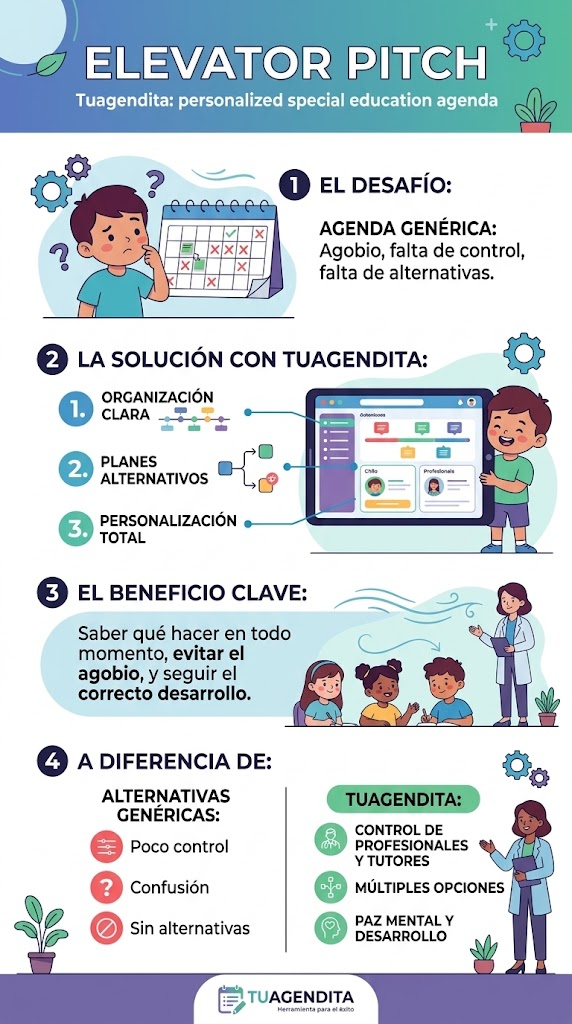
\includegraphics[width=0.62\textwidth]{elevator.png}
\end{center}

\end{document}
